\chapter{Two-reaction system}

At first, the Monte Carlo algorithm implementation was applied to the most basic -- two-reaction test case. We apply it to the model of a plasma composed of three chemical species: argon \ch{Ar},  argon ion \ch{Ar+}, and electron \ch{e-}. Although this system is pretty straightforward, we can use it to illustrate the behavior of our tool and the tasks we will concern ourselves with.

\section{Reactions}

There are only two reactions: argon ionization and recombination. We denote the reaction rates $k_1$ (for argon ionization) and $k_2$ (for recombination).

During the ionization, an electron collides with an electronegative argon atom, causing it to lose an electron:
\ch{e- + Ar ->[ $k_1$ ] e- + e- + Ar+}.

On the other hand, the recombination reaction consists of a ionized argon atom absorbing an electron: 
\ch{e- + Ar+ + Ar ->[ $k_2$ ] Ar + Ar}.

It can be shown that such a system yields an equilibrium, where the electron concentration $\left[ e^{-} \right] = \frac{k_1}{k_2}$ if sufficiently rich in particles. Due to the reaction symmetries, argon ions reach the same concentration; argon atoms then make up the rest of the system.

\section{Deterministic solution}

For this test case, the solution is pretty straightforward. First, we construct the corresponding differential equations for the given reactions. Here, $\left[ X\right]_t$ denotes the concentration of element $X$ at time $t$. 

$$ \frac{\dif \left[ \rm e^{-} \right]_t}{\dif t} = k_1\left[ \rm e^{-}\right]_t \left[ \rm Ar\right]_t - k_2 \left[ \rm e^{-}\right]_t \left[ \rm Ar^{+}\right]_t \left[ \rm Ar\right]_t$$

$$\frac{\dif \left[\rm Ar\right]_t}{\dif t} = - k_1\left[ \rm e^{-}\right]_t \left[ \rm Ar\right]_t + k_2 \left[ \rm e^{-}\right]_t \left[ \rm Ar^{+}\right]_t \left[ \rm Ar\right]_t$$

$$\frac{\dif \left[\rm Ar^{+}\right]_t}{\dif t} = k_1\left[ \rm e^{-}\right]_t \left[ \rm Ar\right]_t - k_2 \left[ \rm e^{-}\right]_t \left[ \rm Ar^{+}\right]_t \left[ \rm Ar\right]_t$$

Note, that the right-hand sides of the differential equations evaluate to zero when we set $\left[ \rm e^{-}\right]_t = \left[\rm Ar^{+}\right]_t = \frac{k_1}{k_2}$. This is the concentration equilibrium of the two-reaction system. 

If we numerically solve these equations, we obtain the result seen on the figure \ref{fig:2reactionBasic}. 
The initial concentrations were chosen to be $\left[e^{-}\right]_0 = \left[Ar^{+}\right]_0 = 1000\;\rm m^{-3}$ and $\left[Ar\right]_0 = 10^{10}\;\rm m^{-3}$. The reaction rates are constant in this case: $k_1 = 10^{-8} \;\rm m^{3} \rm s^{-1}$ and $k_2 = 10^{-12} \;\rm m^{6} \rm s^{-1}$. 

The system reaches an equilibrium precisely at $\left[e^{-}\right]_t = 10^{4}\;\rm m^{-3}$, which is consistent with our expectations.


\section{Monte Carlo solution}

First, we illustrate our stochastic approach on this simple test case. We run the computation for different values of $N$ -- the number of electron superparticles. As explained in the theoretical overview, starting with the electron concentration of 1000$\;$m$^{-3}$, for $N = 10$, each superparticle is of weight 100. The smaller the number of superparticles $N$, the faster the computation is; however, the simulation output is noisier. 

This trend can be seen in the figure \ref{fig:2reactionBasic}, which illustrates the effect of distinct $N$ on the algorithm outcome. At the same time, we can compare the results with the numerical solution. Note that in this particular case, the setting of $N = 1000$ corresponds to the simple Monte Carlo with no reaction or specie weights.

\begin{figure}
    \centering
    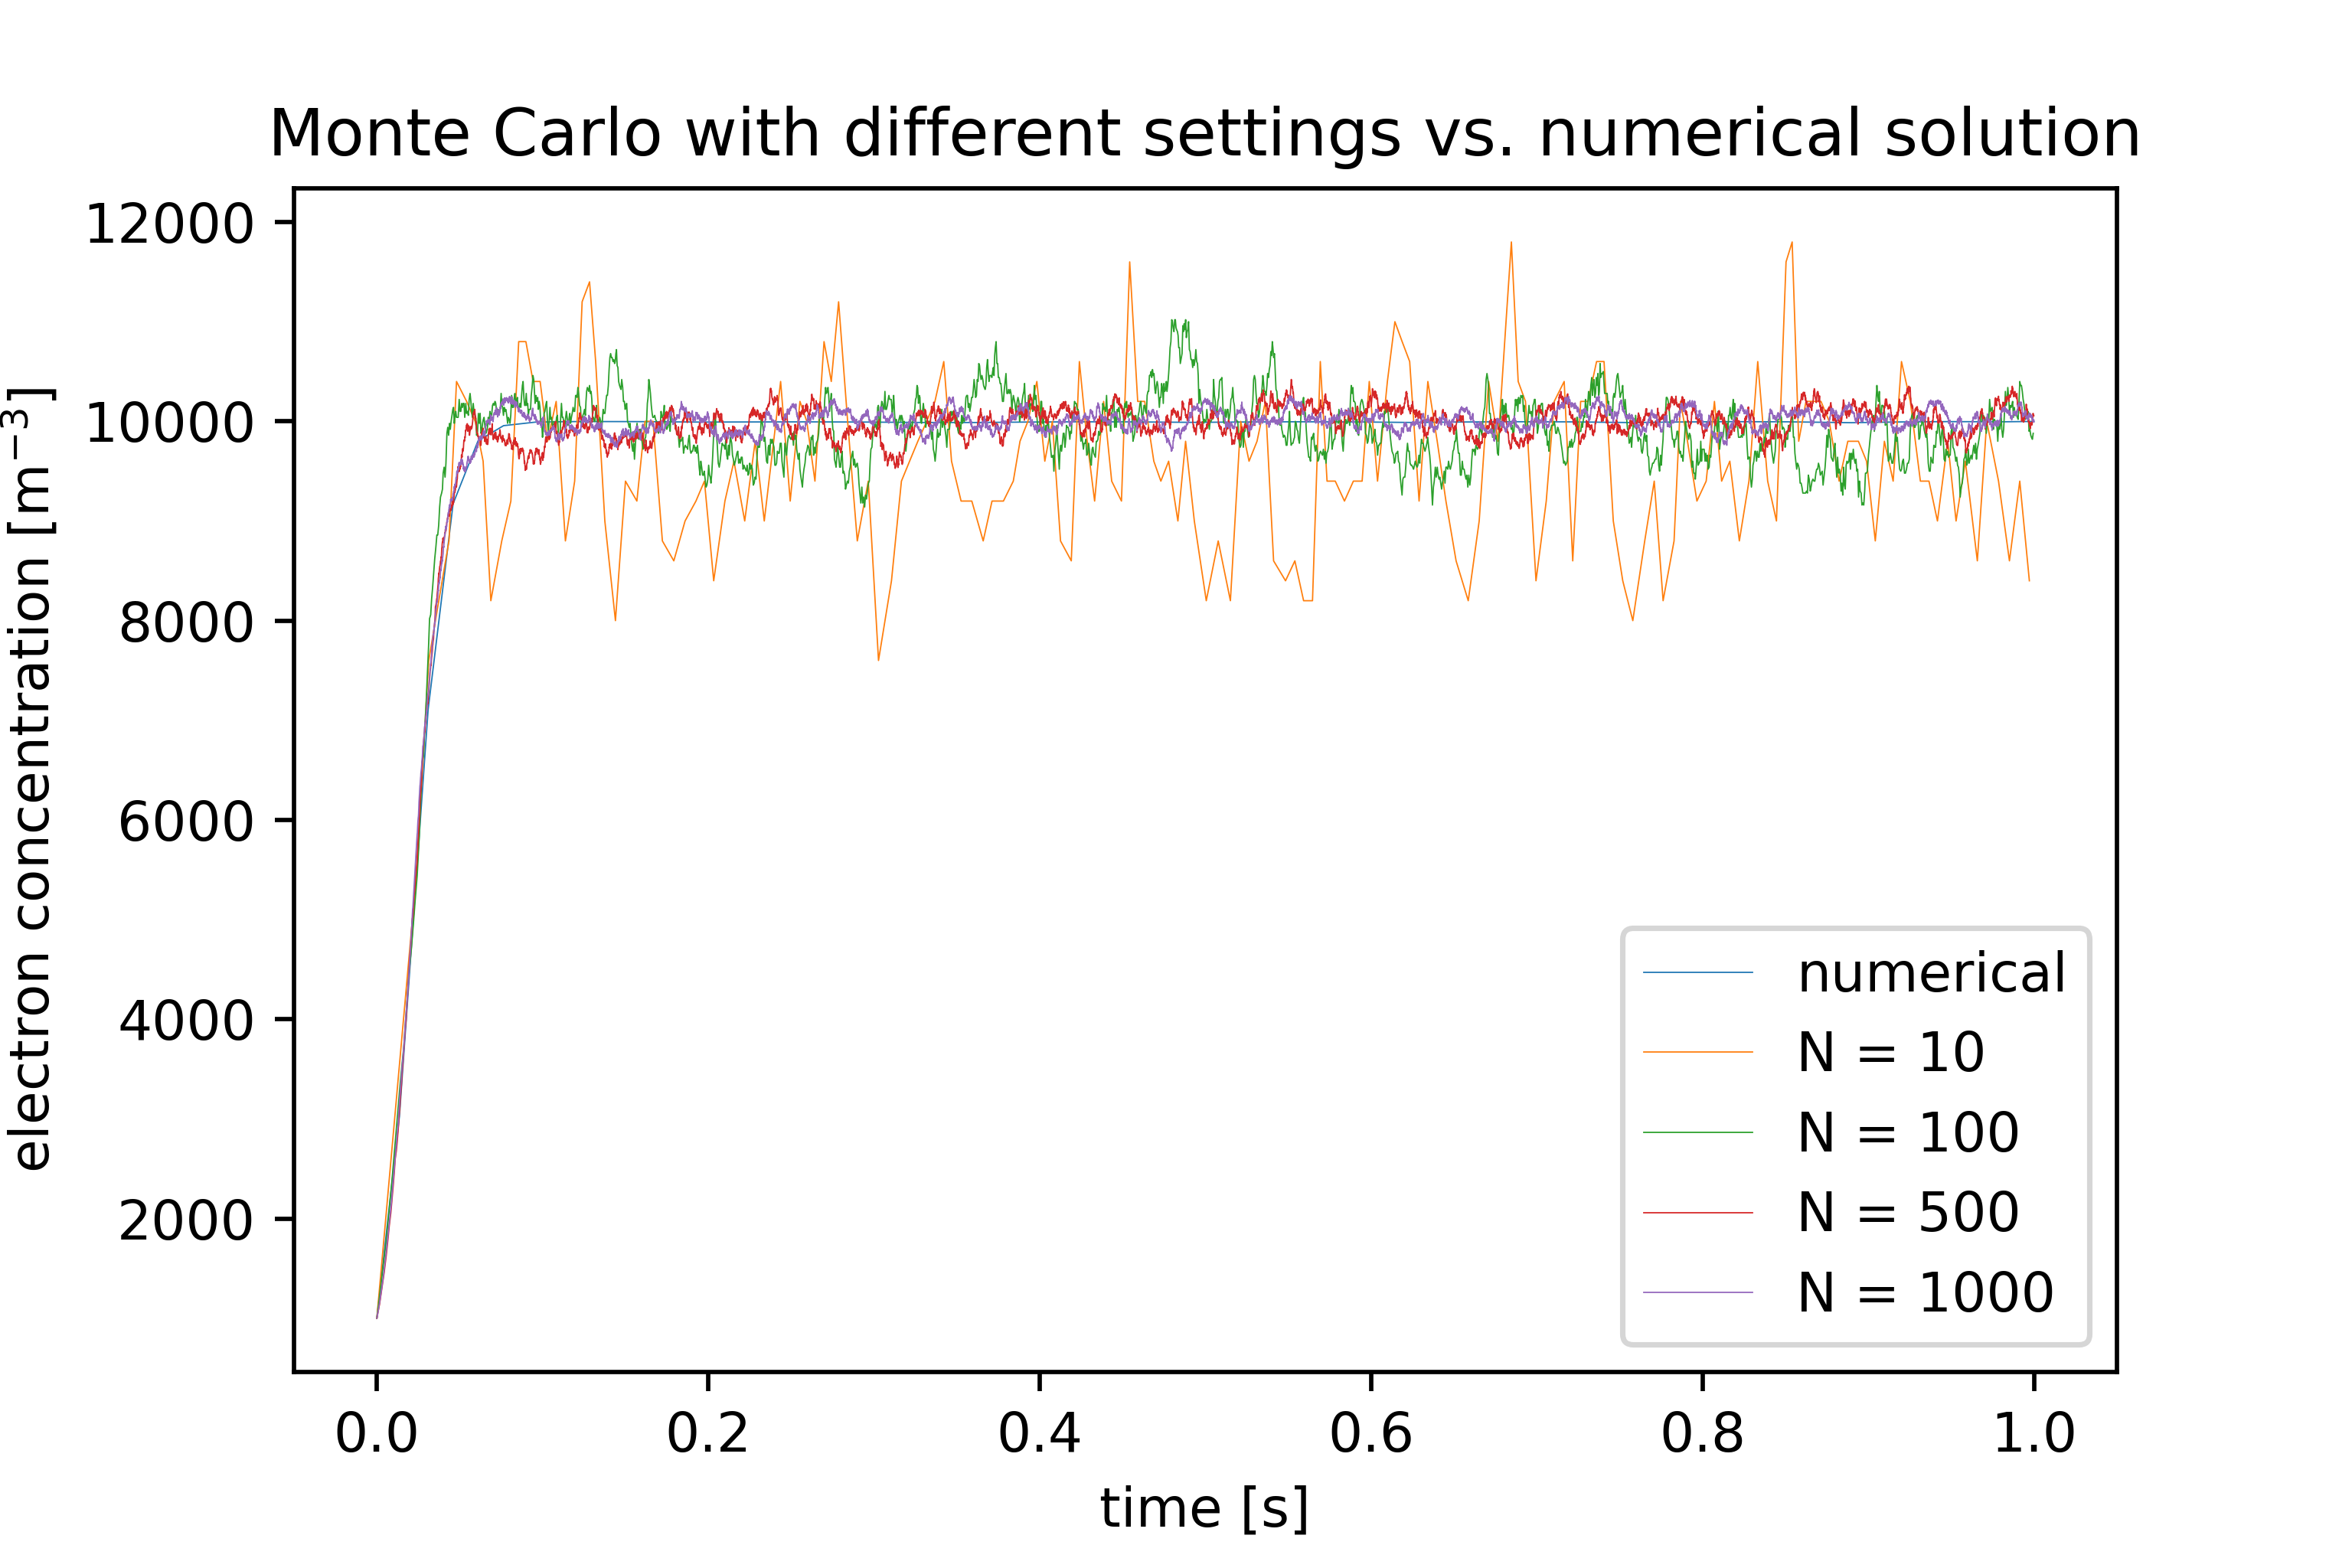
\includegraphics[width=\textwidth]{grafy/2reaction_differentN.png}
    \caption{Two-reaction system -- Monte Carlo with different settings vs. numerical deterministic solution}
    \label{fig:2reactionBasic}
\end{figure}

As mentioned before, the initial concentrations in the simulation were chosen to be $\left[e^{-}\right]_0 = \left[Ar^{+}\right]_0 = 1000\;\rm m^{-3}$ and $\left[Ar\right]_0 = 10^{10}\;\rm m^{-3}$. The reaction rates are constant: $k_1 = 10^{-8} \;\rm m^{3} \rm s^{-1}$ and $k_2 = 10^{-12} \;\rm m^{6} \rm s^{-1}$. 

\subsection{Variable reaction rates}

The algorithm is capable of handling variable reaction rates as well. An example best illustrates this. Let us consider the ionization rate $k_1$ dependent on the value of the reduced electric field $E/N$ as given by the table \ref{tab:ENramp}.

\begin{table}[]
\begin{tabular}{@{}lllll@{}}
\toprule
$t$ [s] & $E/N$ [Td] & $k_1$ [$10^{-8} \rm m^{3} \rm s^{-1}$] & $k_2$ [$10^{-12} \rm m^{6} \rm s^{-1}$] & $\left[ e^{-} \right]_t$ at equilibrium [$\rm m^{-3}$] \\ \midrule
0 -- 1  & 50         & 1.7                                    & 1                                       & 17,000                                                 \\
1 -- 2  & 20         & 1                                      & 1                                       & 10,000                                                 \\
2 -- 3  & 40         & 1.5                                    & 1                                       & 15,000                                                 \\ \bottomrule
\end{tabular}
\caption{Simulation settings for variable ionization rate and theoretical equilibrium electron concentrations}
\label{tab:ENramp}
\end{table}


The outcome of the simulation can be seen in figure \ref{fig:ENramp}. Whenever the ionization rate changes, the electron concentration quickly changes back to its current equilibrium value. While this is undoubtedly a very trivial example of variable reaction rates, it is included here for its simplicity. We will consider and model much more complex systems later.

\begin{figure} 
    \centering
    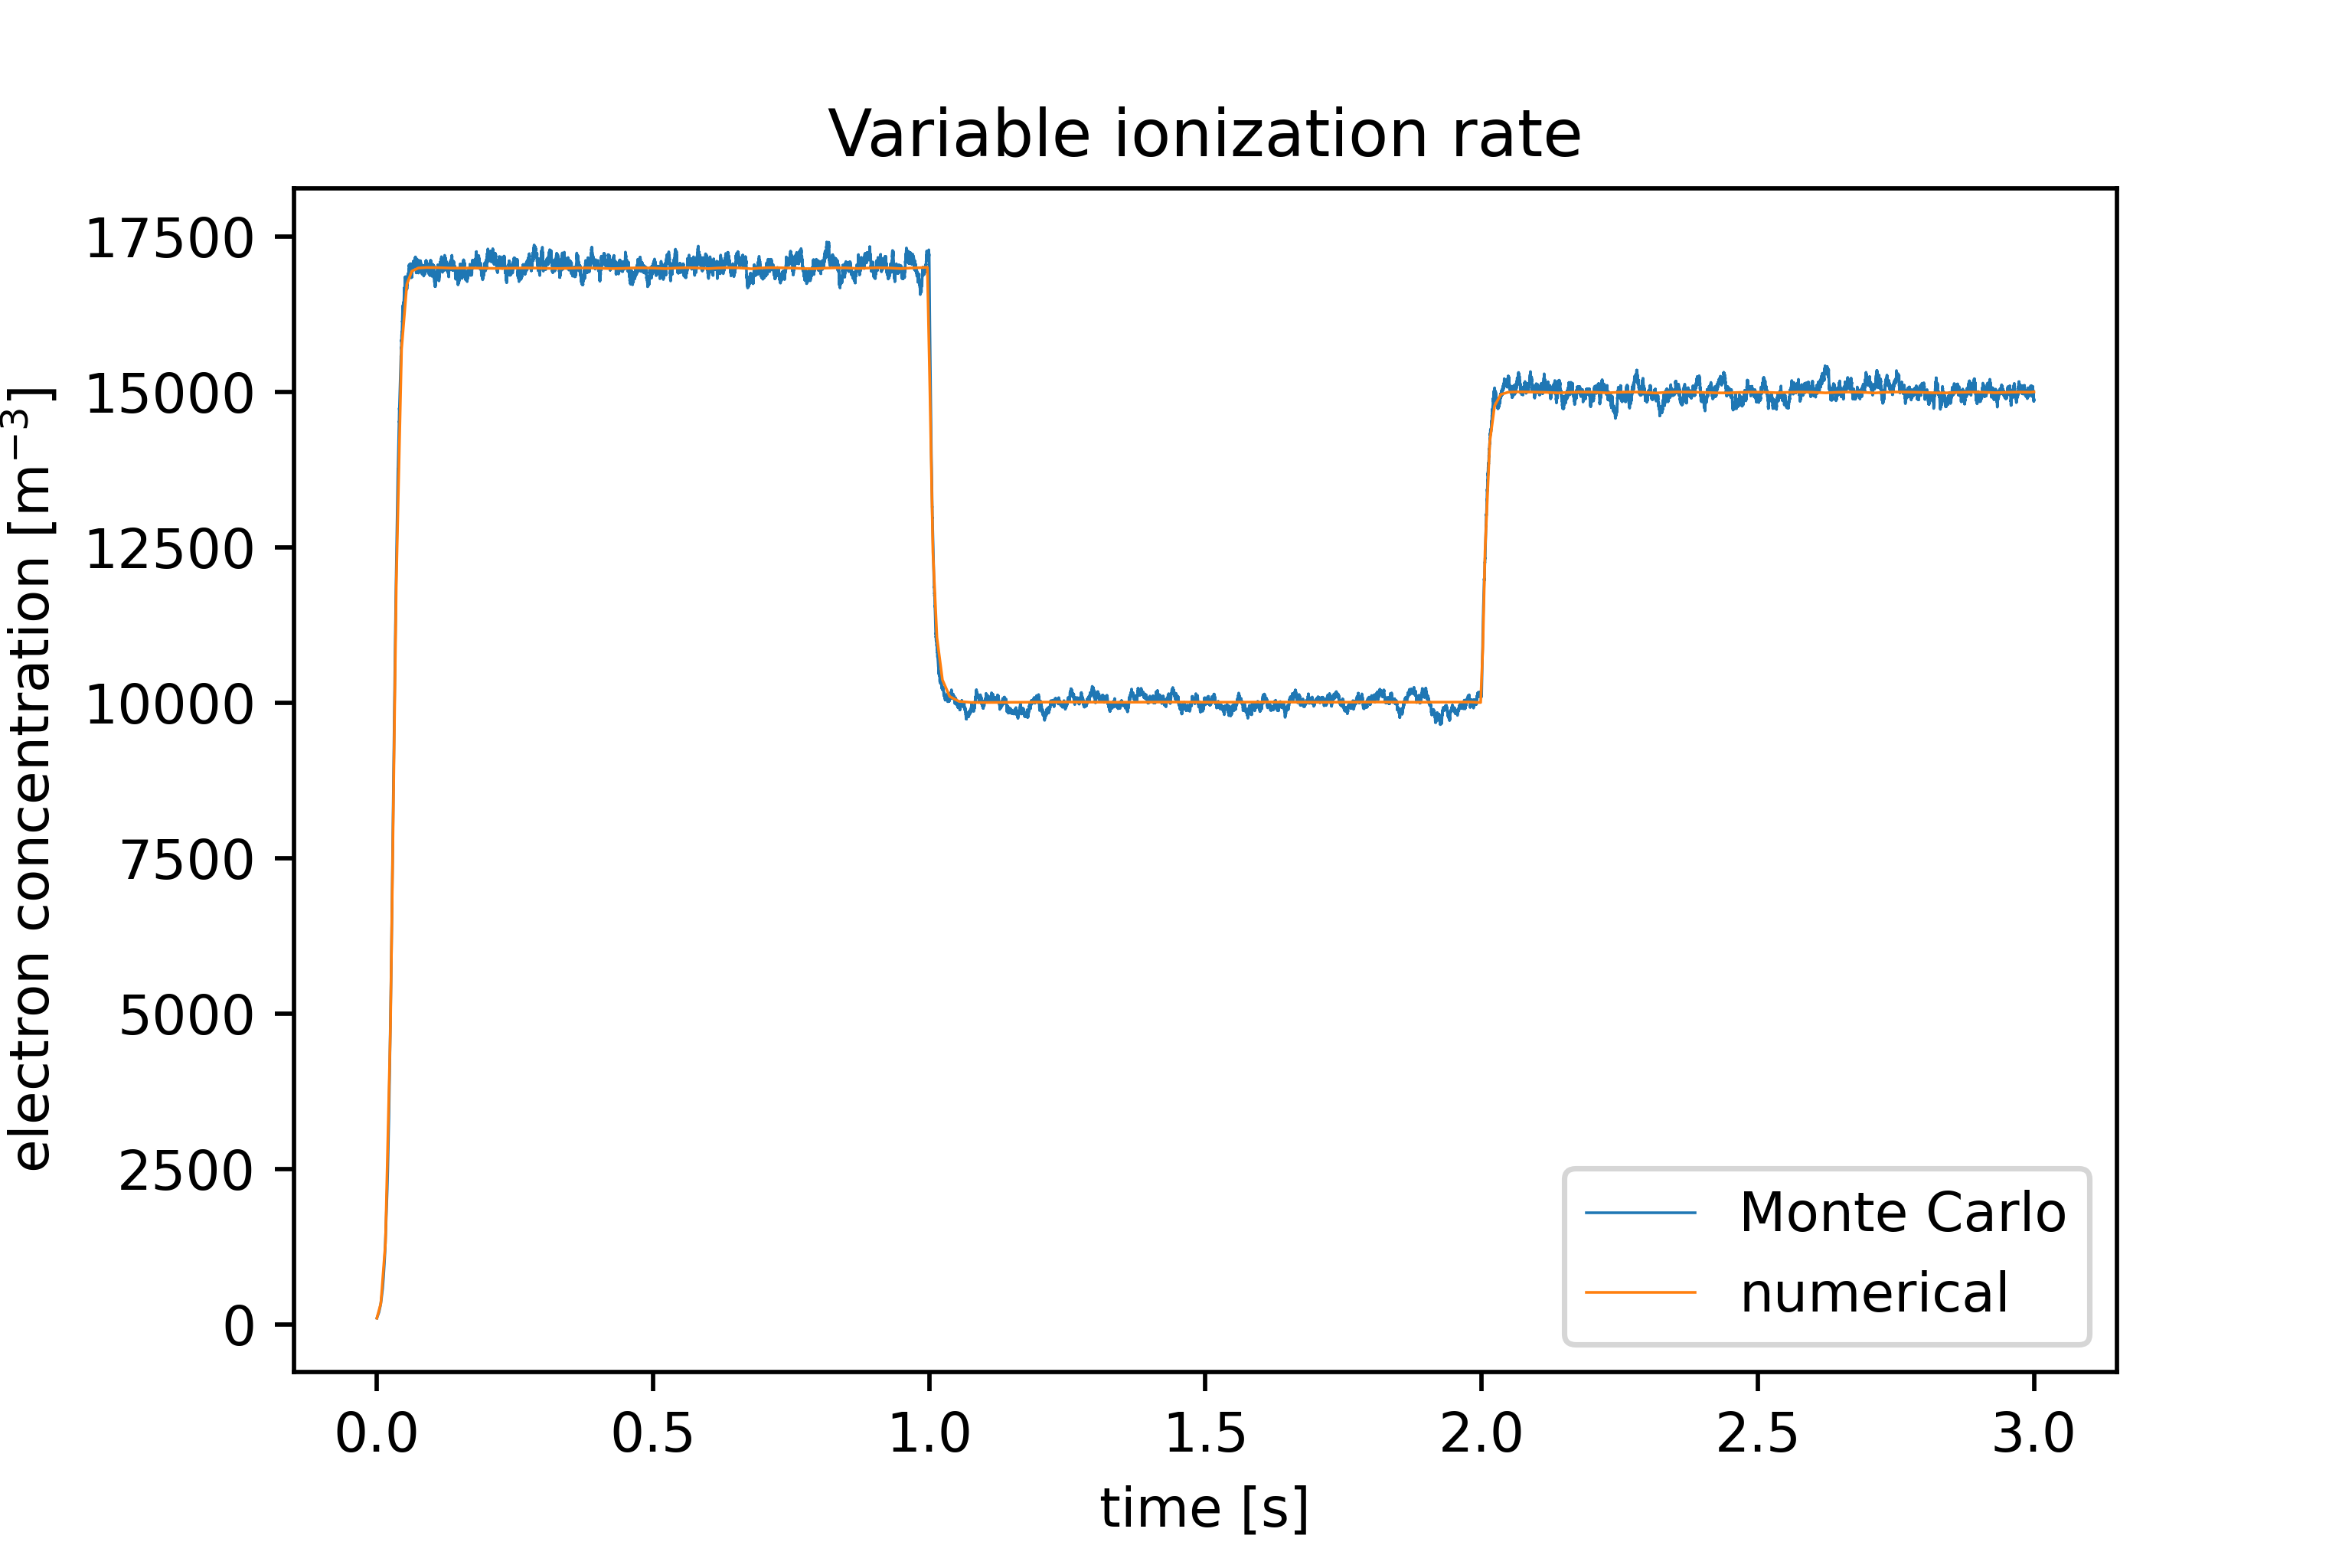
\includegraphics[width=\textwidth]{grafy/ENramp.png}
    \caption{Two-reaction system -- Monte Carlo with variable reaction rates}
    \label{fig:ENramp}
\end{figure}

\subsection{Recalculating superparticle weights}

In the previous simulations, the number of superparticles representing electrons $N$ would change significantly. This is because the superparticle (or reaction) weight $b$ is kept constant during the whole computation, even though the number of particles (and thus also the superparticles representing them) might grow significantly.

For example, in the simulation plotted in figure \ref{fig:2reactionBasic}, consider the case of the initial number of electron superparticles $N = 100$. At the end of the simulation, the electron concentration has grown from $1000\;\rm m^{-3}$ to roughly $10,000\;\rm m^{-3}$, meaning that the number of electron superparticles has increased to $1000$. The computation is thus getting increasingly slower, and in some more extreme (yet realistic) initial simulation settings, the solver might become too slow to be practically useful. This could be the case for different reaction rates, yielding an equilibrium at  $\left[e^{-}\right] = 10^6\;\rm m^{-3}$.

We solve this problem by employing bulk recalculation whenever the current number of superparticles overflows (or underflows) a given threshold, keeping it arbitrarily close to the initial value $N$.

In the figure \ref{fig:2recRecomputingN}, we can examine the effects of this approach on the results. While the computation is noticeably faster, we can see significantly more noise in the simulation. Obviously, that is due to lowering the effective number of superparticles considered in total during the computation.

\begin{figure} 
    \centering
    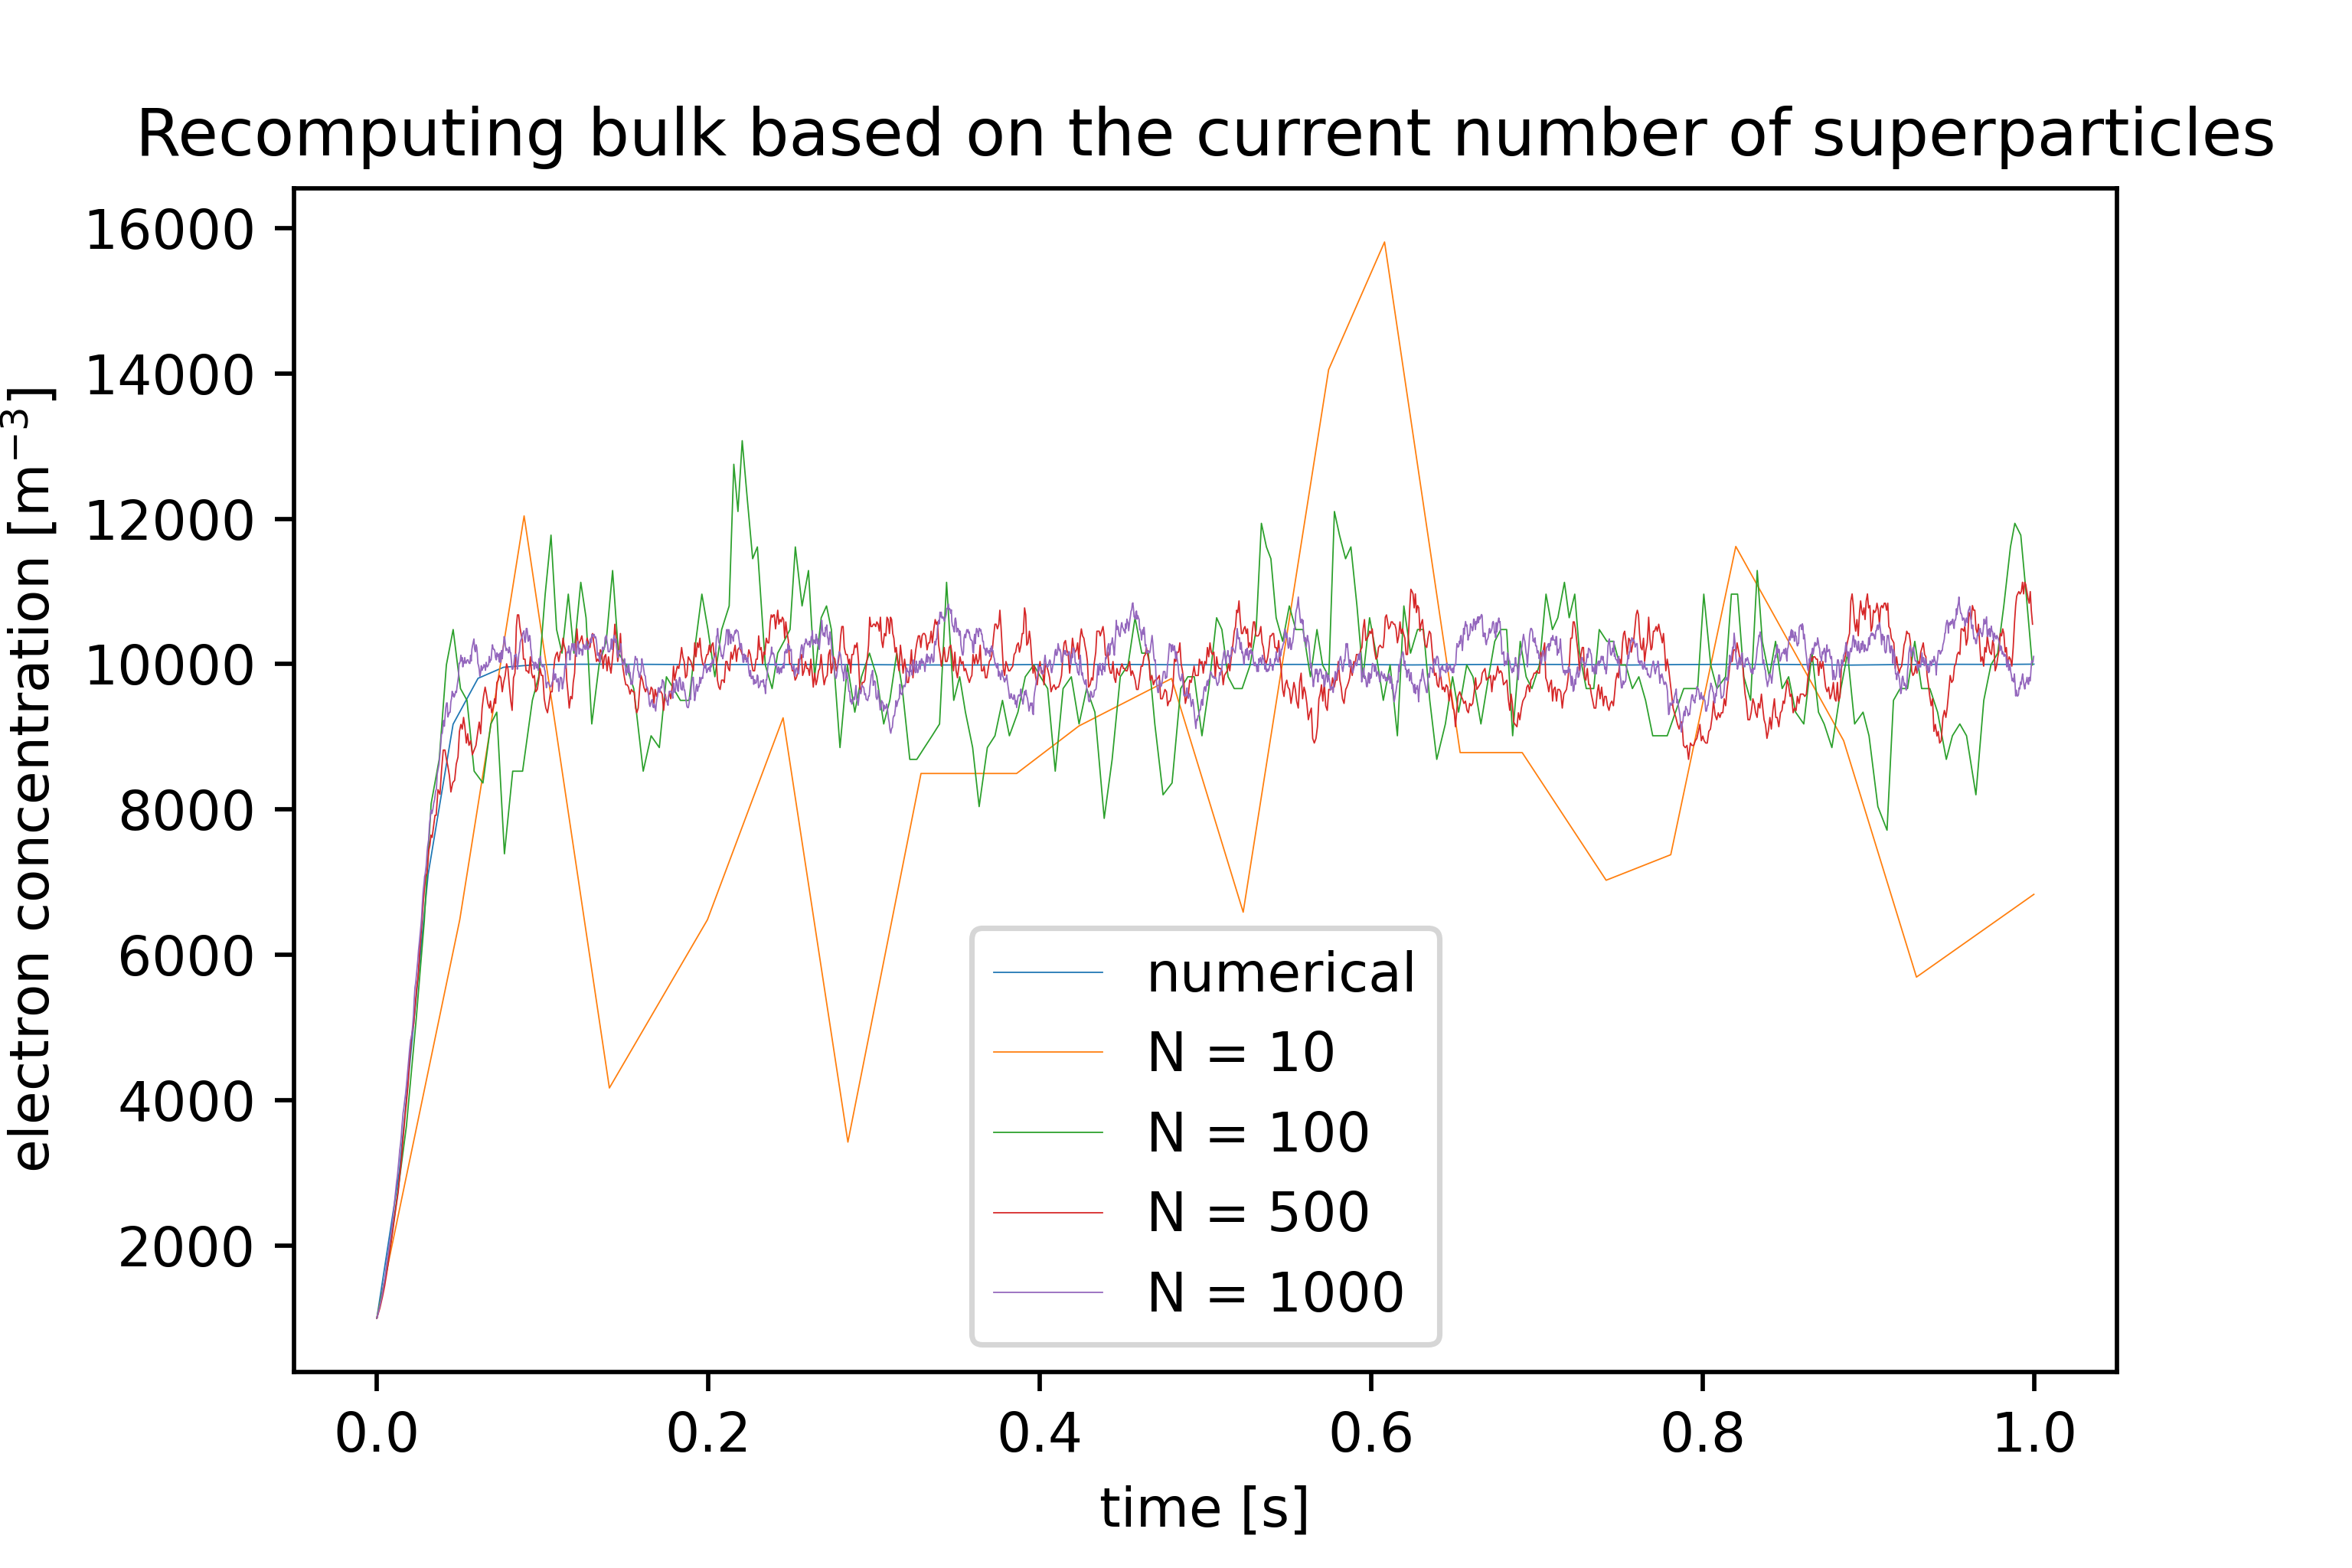
\includegraphics[width=\textwidth]{grafy/2reaction_recomputingN.png}
    \caption{Two-reaction system -- Monte Carlo with bulk recomputing}
    \label{fig:2recRecomputingN}
\end{figure}

\section{Equal reaction weights}

Next, we will use the two reaction test case to explore the equal reaction weights approach. Taking into account a very simple model of two reactions, the presented results are meant to intuitively show the properties of ERW rather than directly proving or disproving its usefulness in practice.

In the figure \ref{fig:2reaction_EqReactionWeights}, we can compare the simple Monte Carlo algorithm, and the simulation output difference when using ERW. The dashed line shows the corresponding numerical solution of the system. The reaction rates are the same as in the previous case: $k_1 = 10^{-8} \;\rm m^{3} \rm s^{-1}$, and $k_2 = 10^{-12} \;\rm m^{6} \rm s^{-1}$. 

\begin{figure} 
    \centering
    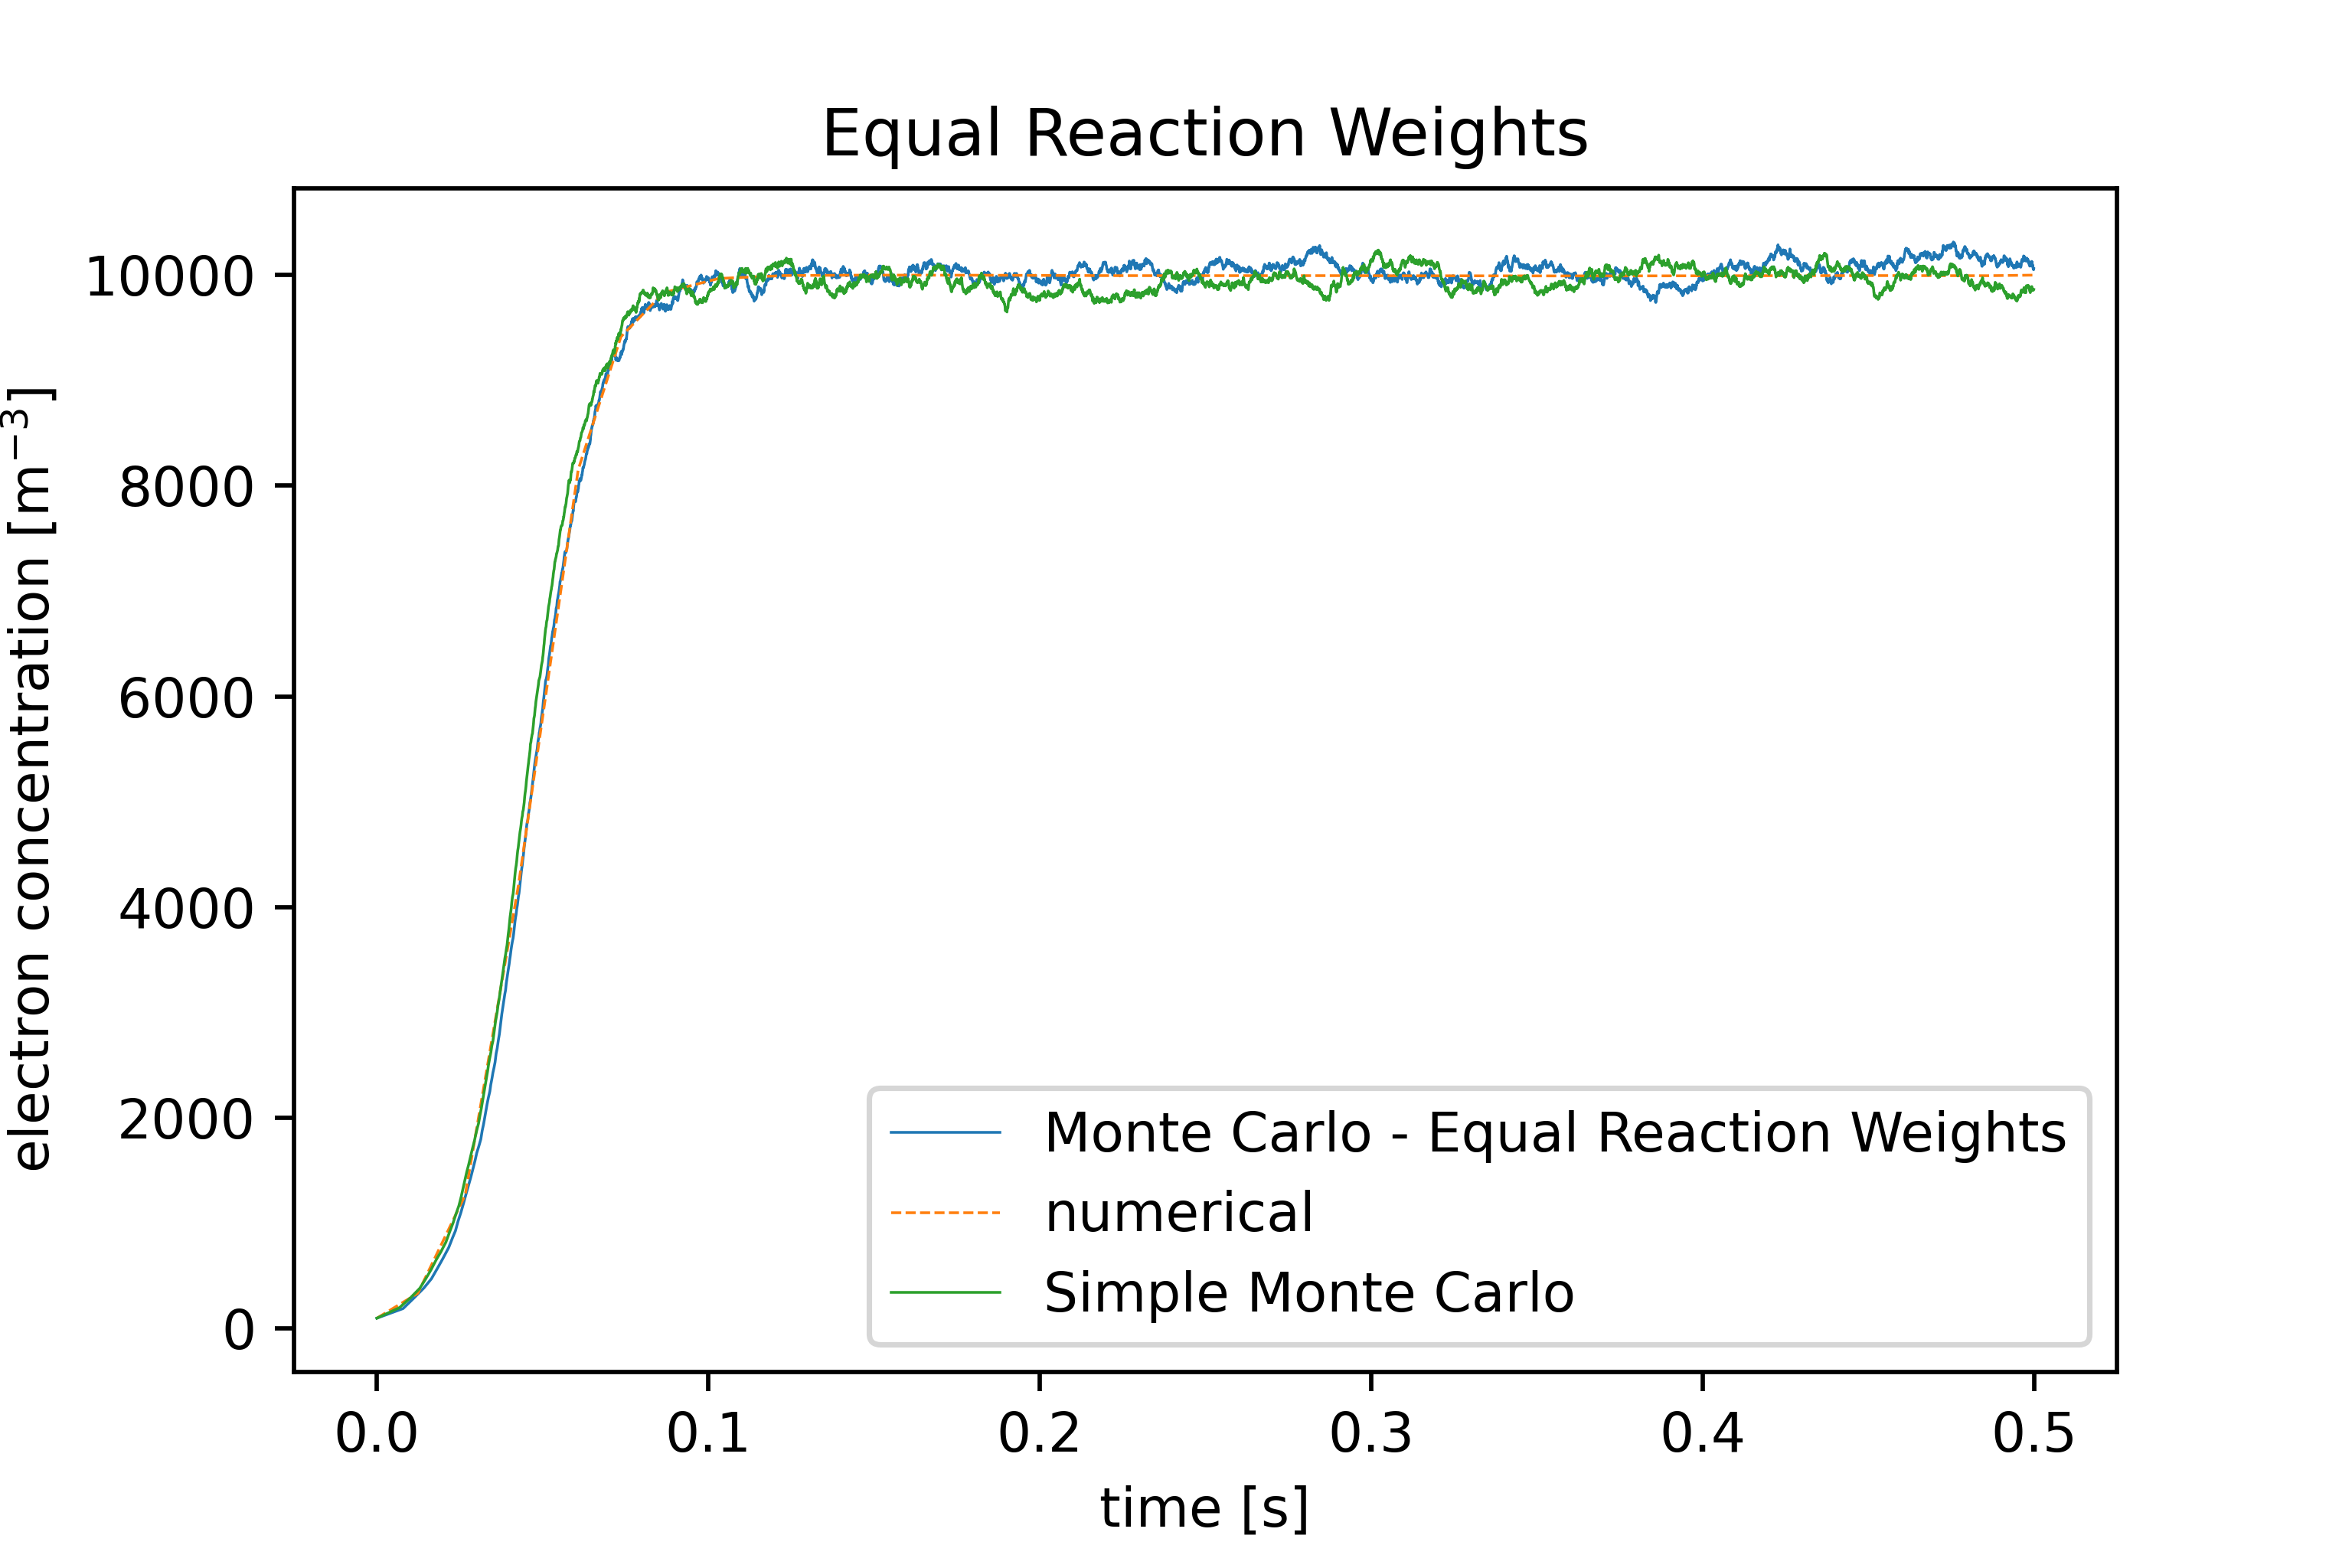
\includegraphics[width=\textwidth]{grafy/2reaction_EqReactionWeights.png}
    \caption{Two-reaction system -- Monte Carlo with equal reaction weights comparison}
    \label{fig:2reaction_EqReactionWeights}
\end{figure}

Clearly, the ERW approach does not seem to have a noticeable impact on the simulation results. That is not a surprising observation; the ERW method proves useful when dealing with rare species concentrations -- which is definitely not the case of electrons, reaching as high as $10^5\;\rm m^{-3}$.

To get a better intuition about the value of the method, we must slightly modify our test case. Because we need a rare species, we will add the reaction \ch{e ->[ $k_3$ ] e(W)}, describing electron diffusion. The new species \ch{e(W)} thus represents electron diffusion loss. We choose $10^{-2}\;\rm s^{-1}$ as the reaction rate $k_3$ value.


\begin{figure} 
    \centering
    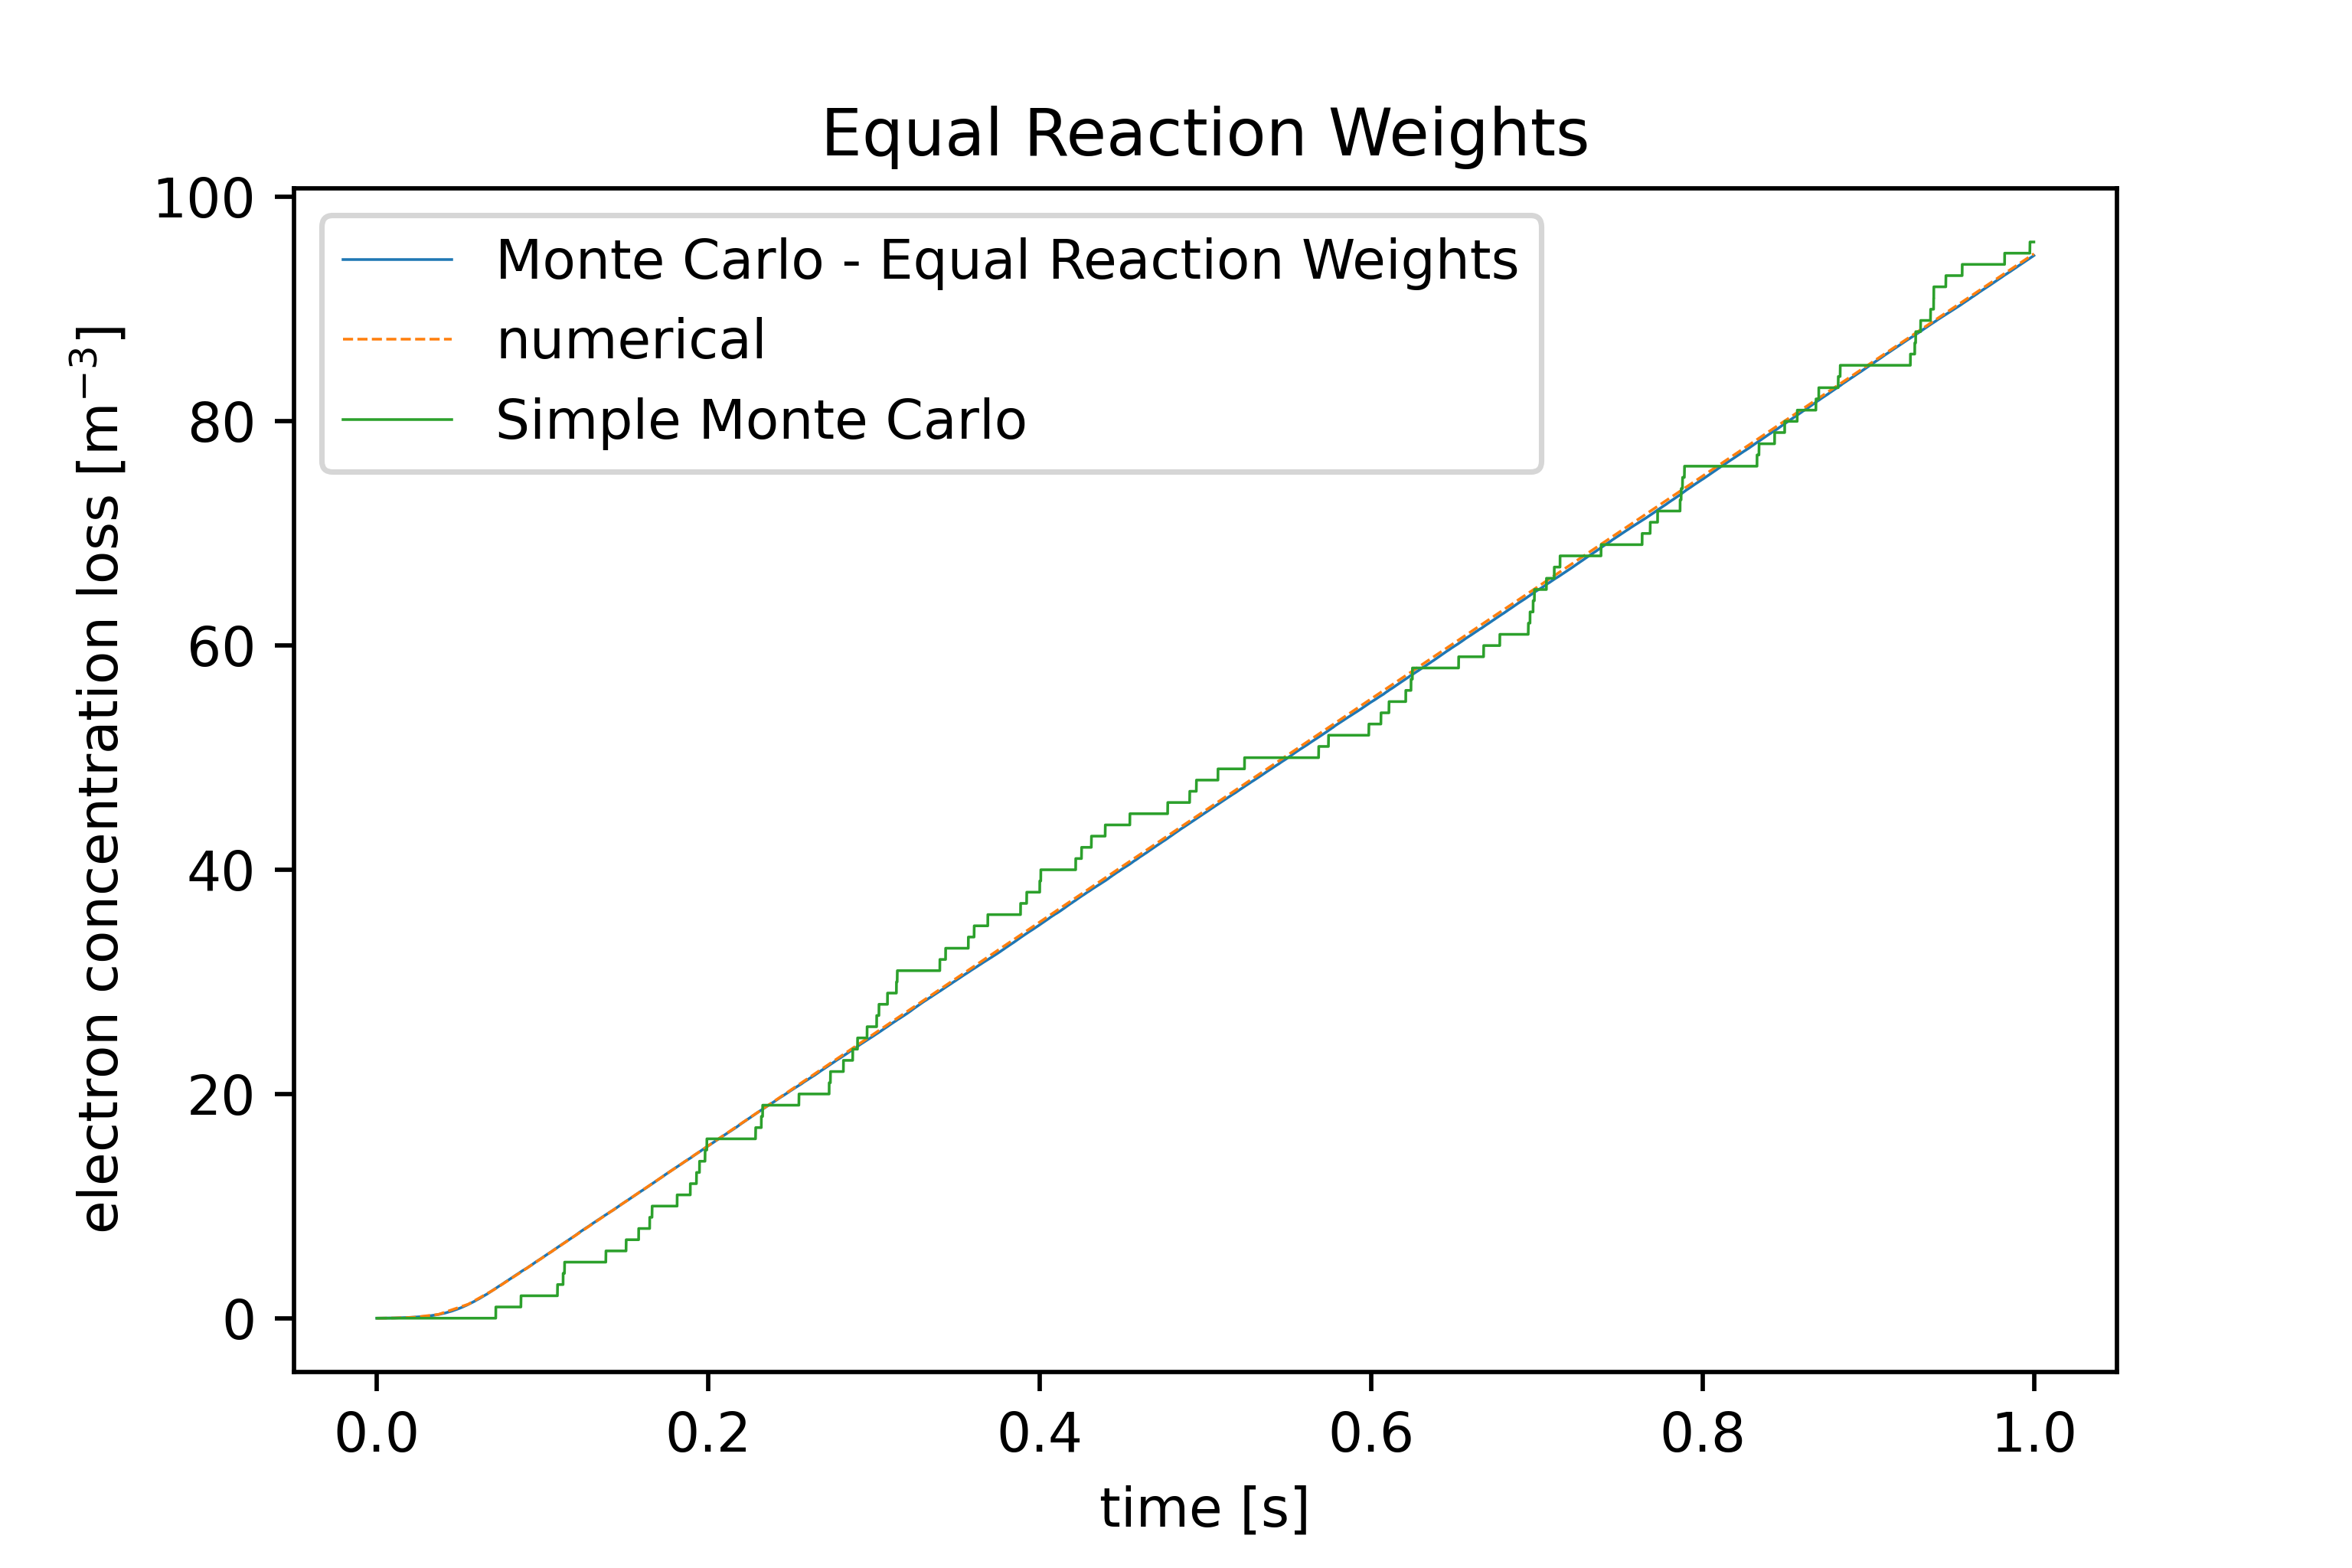
\includegraphics[width=\textwidth]{grafy/EqReactionWeights.png}
    \caption{``Two"-reaction system with electron loss -- Monte Carlo with ERW}
    \label{fig:EqReactionWeights}
\end{figure}

The figure \ref{fig:EqReactionWeights} provides a better illustration of the properties of the ERW approach. As shown, it entirely coincides with the numerical solution of the corresponding differential equations. Note that this is only possible because of its ability to produce fractional particle concentrations, which might not be realistic. The simple Monte Carlo algorithm produces a similar result of integer steps, with a noticeably higher variance.